\section{Process vs thread}
A comparison is provided in Table \ref{tab:thread_vs_process}.
\begin{table}[h]
	\centering
	\resizebox{\textwidth}{!}{%
		\begin{tabular}[\footnotesize]{|m{\textwidth/8}|m{\textwidth/8}|m{\textwidth/6}|m{\textwidth/8}|m{\textwidth/8}|m{\textwidth/5}|}
			\hline
			& \textbf{Memory} & \textbf{Communication} & \textbf{Creation} & \textbf{Control} & \textbf{Changes} \\ \hline
			\textbf{Thread} & Shared address space between threads & Threads can easily communicate between each other via the shared variables & Threads are easily created and destroyed & Threads can exercise considerable control over threads of the same process & Changes to the main thread (cancellation, priority change, etc.) may affect the behavior of the other threads of the process \\ \hline
			\textbf{Process} & Independent address space between processes & Proesses can communicate via considerable overhead with O.S. interprocess communication & Processess require duplication of the parent process & Processes can only exercise control over child processes. & Changes to the parent process do not affect child processes \\ \hline
		\end{tabular}%
	}
	\caption{Thread vs processes}
	\label{tab:thread_vs_process}
\end{table}

\begin{figure}[h]
	\centering
	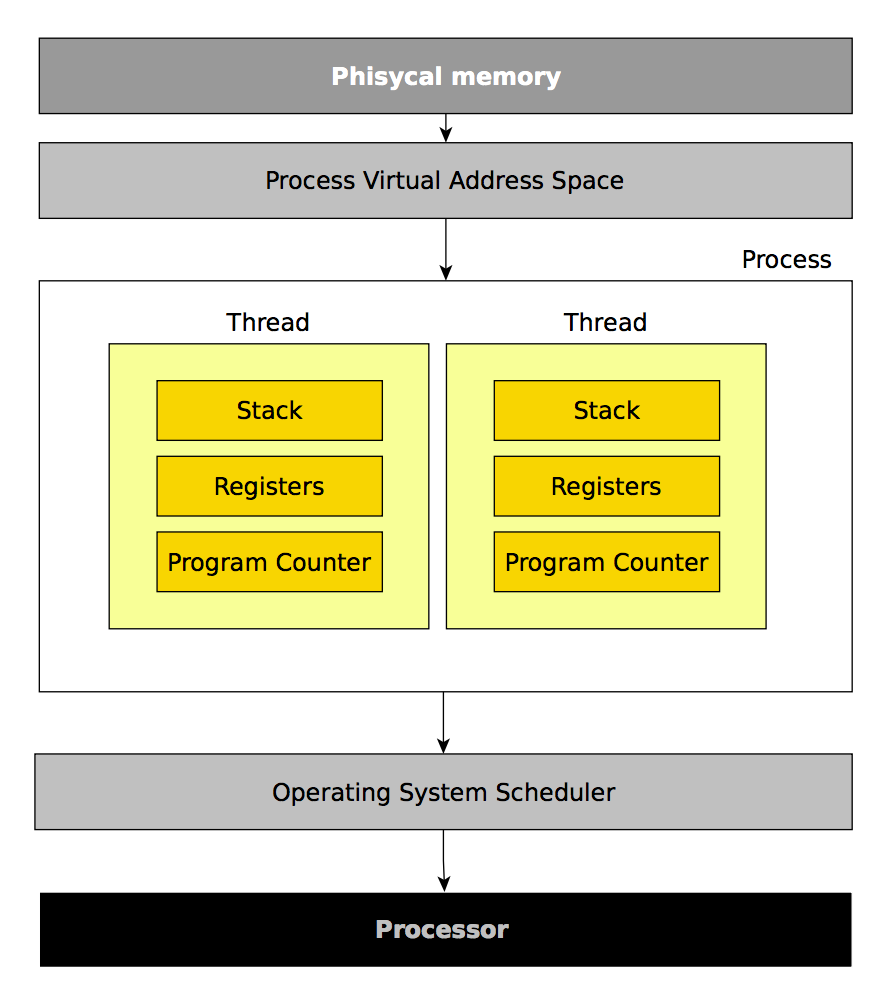
\includegraphics[width=\textwidth/4]{gfx/process_threads}
	
	\caption{Threads in a process}
	\label{Fig:process_threads}
\end{figure}
\section{Operations on processes}

\subsection{fork()}
This command creates a process by duplicating the calling process.
\begin{lstlisting}
#include <stdio.h>

#include <sys/types.h>

#include <unistd.h>
#include <unistd.h>

int main () {
}
return 0; return 0;
}
pid_t child_pid; pid_t child_pid;
printf("Main process id = %d (parent PID = %d)\n",
printf("Main process id = %d (parent PID = %d)\n",
(int) getpid(), (int) getppid()); (int) getpid(), (int) getppid());
child_pid = fork();
child_pid = fork();
if (child_pid != 0) if (child_pid != 0)
else
printf("Parent: child's process id = %d\n", child_pid); printf("Parent: child's process id = %d\n", child_pid);
else
printf("Child: my process id = %d\n", (int) getpid()); printf
\end{lstlisting}
\subsection{title}